\chapter{Quantum Error Correction Codes.}
\section{Introduction.}
It's widely believed that quantum machines have a significant advantage over the classical in the range of computational tasks\cite{grover1996fast}, \cite{ahuja1999quantum}. Simple algorithms could be interpreted as the quantum version of scanning all the options, cutting the running time by the square root of the classical magnitude. 

Nevertheless, Shore has shown a polynomial depth quantum circuit that solves the hidden abelian subgroup \cite{Shor_1997}, which is considered a breakthrough, as it made the computer science community believe that a quantum computer might offer an exponential advantage.

Yet, even though there is a consensus about the superiority of ideal quantum computation model, it is still unclear whether implementing such a machine in the presence of noise is feasible.   
Still, just pointing on the existence of noise is not powerful enough to cancel the feasibility of computation. Evidence of this is that classical computers also suffer from a certain rate of faults. Thus, to fully understand the hardness, let us compare two main reasons that made it realize a hard task. 
First is the magnitude of the error rate, classical computers also have errors, and sometimes we witness system failures (blue screen, for example). The error rate of modern computers is so low that the probability for error to propagate stays negligible even if the length of the computation is polynomial in the scale of what is considered reasonable input size. It's worth mentioning that in exascale computing when supercomputers perform around $10^{18}$ operations per second, It is hard to miss the faults. In quantum, we become aware of their existence much earlier.      

The second difference, which is a tricky point, is that quantum states are sensitive to additional types of error. Along with the chance for bit-flip error, a quantum state might also change its phase. For example, consider the initial state $\ket{+} = \frac{1}{\sqrt{2}}\left( \ket{0} + \ket{1} \right)$, and suppose that due to noise the state transformed into $\frac{1}{\sqrt{4}}\left( \sqrt{3}\ket{0} + \ket{1} \right)$. While classical circuits are blind to such faults. Namely, their run would stay identical as no error occurs. Quantum circuits usually would affect and might fail. Furthermore, when planning a decoder for quantum error correction codes, If one is willing to use a classical code to defend against phase flips, he has to ensure that the decoding doesn't cause bit-flip errors. 
\begin{definition}[Bit and pahse flip.] \label{def:bphf}  
  Consider a quantum state $\ket{\psi}$ encoded in the computation base. We will say that a \textit{bit-flip} occurs in a scenario the operator Pauli $X$ is applied on one of our state's qubits. The bit-flip event could be considered as exactly as the standard bit-flip error in the classical regime. Similarly, \textit{phase-flip} occurs when the Pauli $Z$ is applied on one of the qubits. 

  Notice that together with the identity $I$, the set $\{I, X \otimes e_{i} , Z \otimes e_{j} \}_{i,j \in [n]}$ span the matrices act on $n$ qubits.  
\end{definition}

However, even though quantum noise is so violent, It was proven that any ideal circuit at polynomial depth could be transformed to a robust circuit at poly-logarithmic cost \cite{aharonov1999faulttolerant}. Or in other words, There is a threshold, If the physicists would provide qubits and a finite gate set that suffers from a rate of noise below that threshold, then $BQP$, the class of polynomial time ideal quantum computation is feasible and could be computed on a realistic machine.                

The basic ingredient in \cite{aharonov1999faulttolerant} was to show the existence of quantum error correction code, such that one can perform all the logic operations in a way that restricts present errors from propagating on. That allows them to separate any operation of the computation into stages; one of them is the operation itself, another one is an error correction stage. That process comes with an additional cost, in both space and time, yet it might decrease the probability that the final state at the end would be faulted. The trade-off between the resource needed to pay and the decreasing rate defines the threshold. And if the balance is positive, then one can repeat in a recursion manner, and after log-log iterations, the failure probability decay to zero. At the same time, the circuit would scale at most poly-logarithmic wide and depth factors.      

Let's return to the repetition code presented in Chapter 2. We would like to have an analog; a first and natural attempt might consider duplicating copies of the state. Unfortunately, copying a general state is not a linear operation and therefore can not be done in the circuit model (and any other believed to be feasible). In particular there is no circuit $U$ which duplicate simultaneity the states $\ket{0}, \ket{1}, \ket{+}, \ket{-}$.

To overcome the issue, Shor came up with the nine-quibt code \cite{Ninequ}, which at first glance might seem a naive straightforward implantation of ``duplication'', but instead uses a clever insight about quantumness in general. Any operation can be seen as a linear (and even unitary) operation over a subspace embedded in large enough dimensions. The encoding is given as follow: 
\begin{equation*}
  \begin{split}
    |\overline{0}\rangle&=\frac{1}{2\sqrt{2}}\left(|000\rangle+|111\rangle\right)^{\otimes3}\\
    |\overline{1}\rangle&=\frac{1}{2\sqrt{2}}\left(|000\rangle-|111\rangle\right)^{\otimes3}~.
  \end{split}
\end{equation*}


For convenient let us use the notation, $\ket{\mathbf{GHZ}^{\pm}} =  \ket{0^{m}} \pm  \ket{1^{m}}$. One can also consider the Shor code over $m^{2}$ qubits which defined as above beside that any logical state contain $m$ product over $m$ qubits, So the state $\ket{\overline{0}}$ over $m^{2}$ qubits can be written as $\ket{\mathbf{GHZ}^{+}}^{m}$. We are now ready to prove a statement regards to the robustness.  

\begin{lemma}
  The Shor code over $9$ qubits enable to correct a single either bit or phase flip.  
\end{lemma}
It is evident that a single bit-flip error can be handled in the same way as in the conventional case. The decoder will check if any of the triples have the same value, and if not, it will correct it by majority. To create a decoder that can also correct a phase-flip error, we need the following statement. In this chapter, we denote the Hadamard gate over $m$ qubits as $H^m$.
\begin{claim}
   $H^{m}\ket{\mathbf{GHZ}^{\pm}} = \sum_{ x \cdot \mathbf{1} =_2 \pm }{\ket{x} }$
\end{claim}

\begin{proof}

  \begin{equation*}
    \begin{split}
      H^{m}\ket{\mathbf{GHZ}^{\pm}} & = H^{m}\ket{0^{m}} \pm  H^{m}\ket{1^{m}} = \sum_{x \in \mathbb{F}_{2}^{m}}{\ket{x}} \pm  \sum_{x \in \mathbb{F}_{2}^{m}}{\left( -1 \right)^{x \cdot \mathbf{1}} \ket{x}} \\ & = \sum_{x \in \mathbb{F}_{2}^{m}}{ \left( 1 \pm \left( -1 \right)^{x \cdot \mathbf{1}}  \right) \ket{x} } =  \sum_{x \cdot \mathbf{1} =_2 \pm }{\ket{x} }
    \end{split}
  \end{equation*}
\end{proof}

Now it is clear how to correct a phase flip. One can apply the Hadamard transform and compute the parity of each triple. By the assumption that only a single phase flip may occur, either all the triples have the same parity or the faulted one has an opposite parity and needs to be corrected. Thus, we obtain an $\left[ \left[ 9,1,1 \right] \right]$ quantum error correction code. Asymptotically, this is an $\left[ \left[ m^{2}, 1, m \right] \right]$ code. There is still one big difference between the classic repetition code and the Shor code. While each parity check of the Shor code examines a square root number of qubits, any check of the repetition code touches no more than a constant number of qubits; that is, any check just tests if any two adjacent bits are equal.  That brings us to ask whether the Shors code is really the quantum analogy for the repetition code? 

\paragraph{qLDPC Codes.} As exactly as in the classic case, qLDPC codes are codes in which any check act non trivially on at most a constant number of qubits, It was proved that using a good Quantum LDPC code one can achieve a fault tolerance threshold theorem at the cost of only constant overhead\footnote{under the assumption of holding an efficient decoder.} \cite{gottesman2014faulttolerant}. We are now about to embark on a detailed review of the first quantum LDPC code \cite{Dennis_2002}. 

Recall that one way to present a code is by define the parity check matrix, Consider the $l\times l$ Tours, namely the Cayley graph of the group product  $\mathbb{Z}_{l} \times \mathbb{Z}_{l}$. Associate any coordinate (bit/qubit) with an edge on the Tours. And consider the following two restrictions:

\begin{enumerate}
  \item Each vertex requires form it's local view, the bits lay on his supported edges, To has an even party. 
  \item Each face, requires the almost the same from it's supported edges but that the face compute the parity in different (specific) base. That it, the face is first rotate the qubits by apply the Hadamard transform on them, and than computes their xor. Finally, rotate back the qubits to the computation base.   
\end{enumerate}

\begin{center}
  \begin{figure}[H]
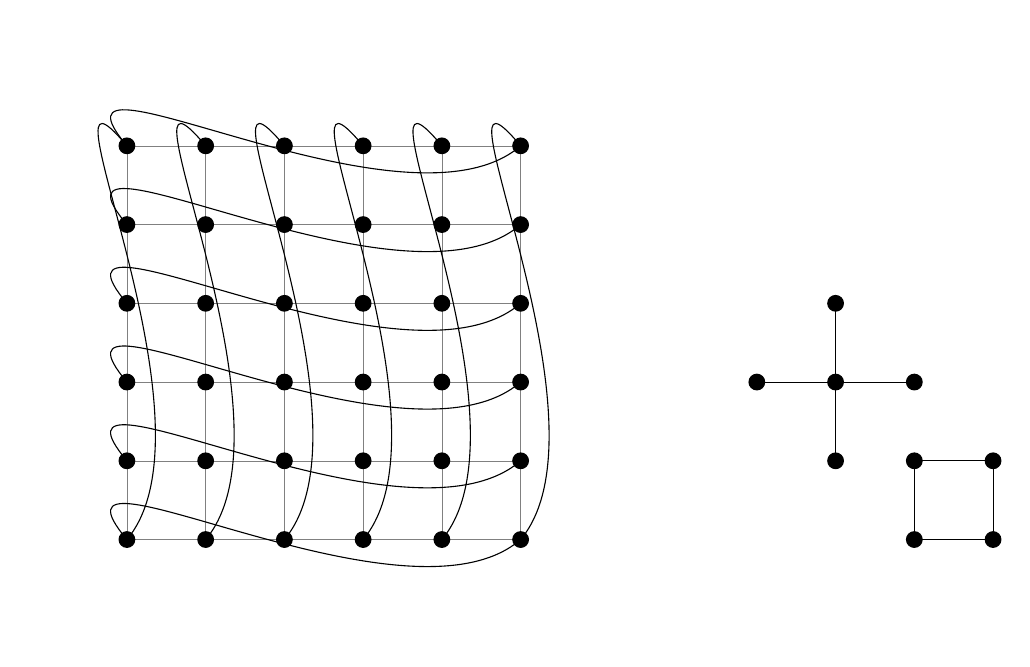
\begin{tikzpicture}
\draw[step=1cm,gray,very thin] (0,0) grid (5,5);
\foreach \x in {0,1,2,3,4,5}
\foreach \y in {0,1,2,3,4,5}
{
\node[draw,circle,inner sep=2pt,fill] at (\x,\y) {};
}
\draw[ -> ]  (0,0) to [out=50, in=130] (0,5);
\draw[ -> ]  (1,0) to [out=50, in=130] (1,5);
\draw[ -> ]  (2,0) to [out=50, in=130] (2,5);
\draw[ -> ]  (3,0) to [out=50, in=130] (3,5);
\draw[ -> ]  (4,0) to [out=50, in=130] (4,5);
\draw[ -> ]  (5,0) to [out=50, in=130] (5,5);
\draw[ -> ]  (0,5) to [out=130, in=220] (5,5);
\draw[ -> ]  (0,4) to [out=130, in=220] (5,4);
\draw[ -> ]  (0,3) to [out=130, in=220] (5,3);
\draw[ -> ]  (0,2) to [out=130, in=220] (5,2);
\draw[ -> ]  (0,1) to [out=130, in=220] (5,1);
\draw[ -> ]  (0,0) to [out=130, in=220] (5,0);

\node[draw,circle,inner sep=2pt,fill] at (9,2) {};
\node[draw,circle,inner sep=2pt,fill] at (10,2) {};
\node[draw,circle,inner sep=2pt,fill] at (8,2) {};
\node[draw,circle,inner sep=2pt,fill] at (9,1) {};
\node[draw,circle,inner sep=2pt,fill] at (9,3) {};
\draw[ -> ]  (9,2) to (10,2);
\draw[ -> ]  (9,2) to (8,2);
\draw[ -> ]  (9,2) to (9,1);
\draw[ -> ]  (9,2) to (9,3);
%\draw[ -> ]  (9,2) to (5,0);

\node[draw,circle,inner sep=2pt,fill] at (10,1) {};
\node[draw,circle,inner sep=2pt,fill] at (11,1) {};
\node[draw,circle,inner sep=2pt,fill] at (10,0) {};
\node[draw,circle,inner sep=2pt,fill] at (11,0) {};
\draw[ -> ]  (10,1) to (11,1);
\draw[ -> ]  (10,1) to (10,0);
\draw[ -> ]  (10,0) to (11,0);
\draw[ -> ]  (11,1) to (11,0);
\end{tikzpicture}
\caption{Toric Graph.}
\label{fig:Toric}
\end{figure}
\end{center}
For example consider some vertex $v$ on the Torus, and let $\ket{\psi} = \sum_{x}{ \ket{\cdots x_{e_0}x_{e_1}x_{e_2}x_{e_3}  \cdots}}$ when $e_{0},e_{1},e_{2},e_{3}$ are the edges compose the local view of $v$. Then in any ket, in the support of $\ket{\psi}$ 


%The Toric code is a topological quantum error-correcting code that encodes a single qubit of information into a two-dimensional lattice of qubits. It is a stabilizer code, meaning that it uses a set of commuting operators to detect and correct errors. The code is based on the mathematical structure of a torus, and its properties make it a powerful tool for quantum computing. It is also a fault-tolerant code, meaning that it can correct errors even when some of the qubits are faulty.
%
%\begin{center}
%  \begin{tikzpicture}
%    \begin{tikzpicture}[scale=1.000000,x=1pt,y=1pt]
\filldraw[color=white] (0.000000, -7.500000) rectangle (240.000000, 217.500000);
% Drawing wires
% Line 1: a0 W
\draw[color=black] (0.000000,210.000000) -- (240.000000,210.000000);
% Line 2: b0 W
\draw[color=black] (0.000000,195.000000) -- (240.000000,195.000000);
% Line 3: c0 W
\draw[color=black] (0.000000,180.000000) -- (240.000000,180.000000);
% Line 4: d0 W
\draw[color=black] (0.000000,165.000000) -- (240.000000,165.000000);
% Line 5: e0 W
\draw[color=black] (0.000000,150.000000) -- (240.000000,150.000000);
% Line 6: a1 W
\draw[color=black] (0.000000,135.000000) -- (240.000000,135.000000);
% Line 7: b1 W
\draw[color=black] (0.000000,120.000000) -- (240.000000,120.000000);
% Line 8: c1 W
\draw[color=black] (0.000000,105.000000) -- (240.000000,105.000000);
% Line 9: d1 W
\draw[color=black] (0.000000,90.000000) -- (240.000000,90.000000);
% Line 10: e1 W
\draw[color=black] (0.000000,75.000000) -- (240.000000,75.000000);
% Line 11: a2 W
\draw[color=black] (0.000000,60.000000) -- (240.000000,60.000000);
% Line 12: b2 W
\draw[color=black] (0.000000,45.000000) -- (240.000000,45.000000);
% Line 13: c2 W
\draw[color=black] (0.000000,30.000000) -- (240.000000,30.000000);
% Line 14: d2 W
\draw[color=black] (0.000000,15.000000) -- (240.000000,15.000000);
% Line 15: e2 W
\draw[color=black] (0.000000,0.000000) -- (240.000000,0.000000);
% Done with wires; drawing gates
% Line 18: d0 C a0
\draw (9.000000,210.000000) -- (9.000000,165.000000);
\begin{scope}
\draw[fill=white] (9.000000, 165.000000) circle(3.000000pt);
\clip (9.000000, 165.000000) circle(3.000000pt);
\draw (6.000000, 165.000000) -- (12.000000, 165.000000);
\draw (9.000000, 162.000000) -- (9.000000, 168.000000);
\end{scope}
\filldraw (9.000000, 210.000000) circle(1.500000pt);
% Line 30: d1 C a1
\draw (9.000000,135.000000) -- (9.000000,90.000000);
\begin{scope}
\draw[fill=white] (9.000000, 90.000000) circle(3.000000pt);
\clip (9.000000, 90.000000) circle(3.000000pt);
\draw (6.000000, 90.000000) -- (12.000000, 90.000000);
\draw (9.000000, 87.000000) -- (9.000000, 93.000000);
\end{scope}
\filldraw (9.000000, 135.000000) circle(1.500000pt);
% Line 42: d2 C a2
\draw (9.000000,60.000000) -- (9.000000,15.000000);
\begin{scope}
\draw[fill=white] (9.000000, 15.000000) circle(3.000000pt);
\clip (9.000000, 15.000000) circle(3.000000pt);
\draw (6.000000, 15.000000) -- (12.000000, 15.000000);
\draw (9.000000, 12.000000) -- (9.000000, 18.000000);
\end{scope}
\filldraw (9.000000, 60.000000) circle(1.500000pt);
% Line 19: d0 C b0
\draw (27.000000,195.000000) -- (27.000000,165.000000);
\begin{scope}
\draw[fill=white] (27.000000, 165.000000) circle(3.000000pt);
\clip (27.000000, 165.000000) circle(3.000000pt);
\draw (24.000000, 165.000000) -- (30.000000, 165.000000);
\draw (27.000000, 162.000000) -- (27.000000, 168.000000);
\end{scope}
\filldraw (27.000000, 195.000000) circle(1.500000pt);
% Line 31: d1 C b1
\draw (27.000000,120.000000) -- (27.000000,90.000000);
\begin{scope}
\draw[fill=white] (27.000000, 90.000000) circle(3.000000pt);
\clip (27.000000, 90.000000) circle(3.000000pt);
\draw (24.000000, 90.000000) -- (30.000000, 90.000000);
\draw (27.000000, 87.000000) -- (27.000000, 93.000000);
\end{scope}
\filldraw (27.000000, 120.000000) circle(1.500000pt);
% Line 43: d2 C b2
\draw (27.000000,45.000000) -- (27.000000,15.000000);
\begin{scope}
\draw[fill=white] (27.000000, 15.000000) circle(3.000000pt);
\clip (27.000000, 15.000000) circle(3.000000pt);
\draw (24.000000, 15.000000) -- (30.000000, 15.000000);
\draw (27.000000, 12.000000) -- (27.000000, 18.000000);
\end{scope}
\filldraw (27.000000, 45.000000) circle(1.500000pt);
% Line 20: e0 C b0
\draw (45.000000,195.000000) -- (45.000000,150.000000);
\begin{scope}
\draw[fill=white] (45.000000, 150.000000) circle(3.000000pt);
\clip (45.000000, 150.000000) circle(3.000000pt);
\draw (42.000000, 150.000000) -- (48.000000, 150.000000);
\draw (45.000000, 147.000000) -- (45.000000, 153.000000);
\end{scope}
\filldraw (45.000000, 195.000000) circle(1.500000pt);
% Line 32: e1 C b1
\draw (45.000000,120.000000) -- (45.000000,75.000000);
\begin{scope}
\draw[fill=white] (45.000000, 75.000000) circle(3.000000pt);
\clip (45.000000, 75.000000) circle(3.000000pt);
\draw (42.000000, 75.000000) -- (48.000000, 75.000000);
\draw (45.000000, 72.000000) -- (45.000000, 78.000000);
\end{scope}
\filldraw (45.000000, 120.000000) circle(1.500000pt);
% Line 44: e2 C b2
\draw (45.000000,45.000000) -- (45.000000,0.000000);
\begin{scope}
\draw[fill=white] (45.000000, 0.000000) circle(3.000000pt);
\clip (45.000000, 0.000000) circle(3.000000pt);
\draw (42.000000, 0.000000) -- (48.000000, 0.000000);
\draw (45.000000, -3.000000) -- (45.000000, 3.000000);
\end{scope}
\filldraw (45.000000, 45.000000) circle(1.500000pt);
% Line 21: e0 C c0
\draw (63.000000,180.000000) -- (63.000000,150.000000);
\begin{scope}
\draw[fill=white] (63.000000, 150.000000) circle(3.000000pt);
\clip (63.000000, 150.000000) circle(3.000000pt);
\draw (60.000000, 150.000000) -- (66.000000, 150.000000);
\draw (63.000000, 147.000000) -- (63.000000, 153.000000);
\end{scope}
\filldraw (63.000000, 180.000000) circle(1.500000pt);
% Line 33: e1 C c1
\draw (63.000000,105.000000) -- (63.000000,75.000000);
\begin{scope}
\draw[fill=white] (63.000000, 75.000000) circle(3.000000pt);
\clip (63.000000, 75.000000) circle(3.000000pt);
\draw (60.000000, 75.000000) -- (66.000000, 75.000000);
\draw (63.000000, 72.000000) -- (63.000000, 78.000000);
\end{scope}
\filldraw (63.000000, 105.000000) circle(1.500000pt);
% Line 45: e2 C c2
\draw (63.000000,30.000000) -- (63.000000,0.000000);
\begin{scope}
\draw[fill=white] (63.000000, 0.000000) circle(3.000000pt);
\clip (63.000000, 0.000000) circle(3.000000pt);
\draw (60.000000, 0.000000) -- (66.000000, 0.000000);
\draw (63.000000, -3.000000) -- (63.000000, 3.000000);
\end{scope}
\filldraw (63.000000, 30.000000) circle(1.500000pt);
% Line 22: e0 G $X$
\begin{scope}
\draw[fill=white] (84.000000, 150.000000) +(-45.000000:8.485281pt and 8.485281pt) -- +(45.000000:8.485281pt and 8.485281pt) -- +(135.000000:8.485281pt and 8.485281pt) -- +(225.000000:8.485281pt and 8.485281pt) -- cycle;
\clip (84.000000, 150.000000) +(-45.000000:8.485281pt and 8.485281pt) -- +(45.000000:8.485281pt and 8.485281pt) -- +(135.000000:8.485281pt and 8.485281pt) -- +(225.000000:8.485281pt and 8.485281pt) -- cycle;
\draw (84.000000, 150.000000) node {$X$};
\end{scope}
% Line 34: d1 e1 +b1
\draw (84.000000,120.000000) -- (84.000000,75.000000);
\filldraw (84.000000, 90.000000) circle(1.500000pt);
\filldraw (84.000000, 75.000000) circle(1.500000pt);
\begin{scope}
\draw[fill=white] (84.000000, 120.000000) circle(3.000000pt);
\clip (84.000000, 120.000000) circle(3.000000pt);
\draw (81.000000, 120.000000) -- (87.000000, 120.000000);
\draw (84.000000, 117.000000) -- (84.000000, 123.000000);
\end{scope}
% Line 46: d2 e2 +b2
\draw (84.000000,45.000000) -- (84.000000,0.000000);
\filldraw (84.000000, 15.000000) circle(1.500000pt);
\filldraw (84.000000, 0.000000) circle(1.500000pt);
\begin{scope}
\draw[fill=white] (84.000000, 45.000000) circle(3.000000pt);
\clip (84.000000, 45.000000) circle(3.000000pt);
\draw (81.000000, 45.000000) -- (87.000000, 45.000000);
\draw (84.000000, 42.000000) -- (84.000000, 48.000000);
\end{scope}
% Line 23: d0 e0 +c0
\draw (108.000000,180.000000) -- (108.000000,150.000000);
\filldraw (108.000000, 165.000000) circle(1.500000pt);
\filldraw (108.000000, 150.000000) circle(1.500000pt);
\begin{scope}
\draw[fill=white] (108.000000, 180.000000) circle(3.000000pt);
\clip (108.000000, 180.000000) circle(3.000000pt);
\draw (105.000000, 180.000000) -- (111.000000, 180.000000);
\draw (108.000000, 177.000000) -- (108.000000, 183.000000);
\end{scope}
% Line 35: d1 G $X$
\begin{scope}
\draw[fill=white] (108.000000, 90.000000) +(-45.000000:8.485281pt and 8.485281pt) -- +(45.000000:8.485281pt and 8.485281pt) -- +(135.000000:8.485281pt and 8.485281pt) -- +(225.000000:8.485281pt and 8.485281pt) -- cycle;
\clip (108.000000, 90.000000) +(-45.000000:8.485281pt and 8.485281pt) -- +(45.000000:8.485281pt and 8.485281pt) -- +(135.000000:8.485281pt and 8.485281pt) -- +(225.000000:8.485281pt and 8.485281pt) -- cycle;
\draw (108.000000, 90.000000) node {$X$};
\end{scope}
% Line 47: d2 G $X$
\begin{scope}
\draw[fill=white] (108.000000, 15.000000) +(-45.000000:8.485281pt and 8.485281pt) -- +(45.000000:8.485281pt and 8.485281pt) -- +(135.000000:8.485281pt and 8.485281pt) -- +(225.000000:8.485281pt and 8.485281pt) -- cycle;
\clip (108.000000, 15.000000) +(-45.000000:8.485281pt and 8.485281pt) -- +(45.000000:8.485281pt and 8.485281pt) -- +(135.000000:8.485281pt and 8.485281pt) -- +(225.000000:8.485281pt and 8.485281pt) -- cycle;
\draw (108.000000, 15.000000) node {$X$};
\end{scope}
% Line 58: b1 G $H$
\begin{scope}
\draw[fill=white] (108.000000, 120.000000) +(-45.000000:8.485281pt and 8.485281pt) -- +(45.000000:8.485281pt and 8.485281pt) -- +(135.000000:8.485281pt and 8.485281pt) -- +(225.000000:8.485281pt and 8.485281pt) -- cycle;
\clip (108.000000, 120.000000) +(-45.000000:8.485281pt and 8.485281pt) -- +(45.000000:8.485281pt and 8.485281pt) -- +(135.000000:8.485281pt and 8.485281pt) -- +(225.000000:8.485281pt and 8.485281pt) -- cycle;
\draw (108.000000, 120.000000) node {$H$};
\end{scope}
% Line 61: b2 G $H$
\begin{scope}
\draw[fill=white] (108.000000, 45.000000) +(-45.000000:8.485281pt and 8.485281pt) -- +(45.000000:8.485281pt and 8.485281pt) -- +(135.000000:8.485281pt and 8.485281pt) -- +(225.000000:8.485281pt and 8.485281pt) -- cycle;
\clip (108.000000, 45.000000) +(-45.000000:8.485281pt and 8.485281pt) -- +(45.000000:8.485281pt and 8.485281pt) -- +(135.000000:8.485281pt and 8.485281pt) -- +(225.000000:8.485281pt and 8.485281pt) -- cycle;
\draw (108.000000, 45.000000) node {$H$};
\end{scope}
% Line 24: e0 G $X$
\begin{scope}
\draw[fill=white] (132.000000, 150.000000) +(-45.000000:8.485281pt and 8.485281pt) -- +(45.000000:8.485281pt and 8.485281pt) -- +(135.000000:8.485281pt and 8.485281pt) -- +(225.000000:8.485281pt and 8.485281pt) -- cycle;
\clip (132.000000, 150.000000) +(-45.000000:8.485281pt and 8.485281pt) -- +(45.000000:8.485281pt and 8.485281pt) -- +(135.000000:8.485281pt and 8.485281pt) -- +(225.000000:8.485281pt and 8.485281pt) -- cycle;
\draw (132.000000, 150.000000) node {$X$};
\end{scope}
% Line 36: d1 e1 +a1
\draw (132.000000,135.000000) -- (132.000000,75.000000);
\filldraw (132.000000, 90.000000) circle(1.500000pt);
\filldraw (132.000000, 75.000000) circle(1.500000pt);
\begin{scope}
\draw[fill=white] (132.000000, 135.000000) circle(3.000000pt);
\clip (132.000000, 135.000000) circle(3.000000pt);
\draw (129.000000, 135.000000) -- (135.000000, 135.000000);
\draw (132.000000, 132.000000) -- (132.000000, 138.000000);
\end{scope}
% Line 48: d2 e2 +a2
\draw (132.000000,60.000000) -- (132.000000,0.000000);
\filldraw (132.000000, 15.000000) circle(1.500000pt);
\filldraw (132.000000, 0.000000) circle(1.500000pt);
\begin{scope}
\draw[fill=white] (132.000000, 60.000000) circle(3.000000pt);
\clip (132.000000, 60.000000) circle(3.000000pt);
\draw (129.000000, 60.000000) -- (135.000000, 60.000000);
\draw (132.000000, 57.000000) -- (132.000000, 63.000000);
\end{scope}
% Line 56: c0 G $H$
\begin{scope}
\draw[fill=white] (132.000000, 180.000000) +(-45.000000:8.485281pt and 8.485281pt) -- +(45.000000:8.485281pt and 8.485281pt) -- +(135.000000:8.485281pt and 8.485281pt) -- +(225.000000:8.485281pt and 8.485281pt) -- cycle;
\clip (132.000000, 180.000000) +(-45.000000:8.485281pt and 8.485281pt) -- +(45.000000:8.485281pt and 8.485281pt) -- +(135.000000:8.485281pt and 8.485281pt) -- +(225.000000:8.485281pt and 8.485281pt) -- cycle;
\draw (132.000000, 180.000000) node {$H$};
\end{scope}
% Line 25: d0 e0 +b0
\draw (156.000000,195.000000) -- (156.000000,150.000000);
\filldraw (156.000000, 165.000000) circle(1.500000pt);
\filldraw (156.000000, 150.000000) circle(1.500000pt);
\begin{scope}
\draw[fill=white] (156.000000, 195.000000) circle(3.000000pt);
\clip (156.000000, 195.000000) circle(3.000000pt);
\draw (153.000000, 195.000000) -- (159.000000, 195.000000);
\draw (156.000000, 192.000000) -- (156.000000, 198.000000);
\end{scope}
% Line 37: d1 G $X$
\begin{scope}
\draw[fill=white] (156.000000, 90.000000) +(-45.000000:8.485281pt and 8.485281pt) -- +(45.000000:8.485281pt and 8.485281pt) -- +(135.000000:8.485281pt and 8.485281pt) -- +(225.000000:8.485281pt and 8.485281pt) -- cycle;
\clip (156.000000, 90.000000) +(-45.000000:8.485281pt and 8.485281pt) -- +(45.000000:8.485281pt and 8.485281pt) -- +(135.000000:8.485281pt and 8.485281pt) -- +(225.000000:8.485281pt and 8.485281pt) -- cycle;
\draw (156.000000, 90.000000) node {$X$};
\end{scope}
% Line 38: e1 G $X$
\begin{scope}
\draw[fill=white] (156.000000, 75.000000) +(-45.000000:8.485281pt and 8.485281pt) -- +(45.000000:8.485281pt and 8.485281pt) -- +(135.000000:8.485281pt and 8.485281pt) -- +(225.000000:8.485281pt and 8.485281pt) -- cycle;
\clip (156.000000, 75.000000) +(-45.000000:8.485281pt and 8.485281pt) -- +(45.000000:8.485281pt and 8.485281pt) -- +(135.000000:8.485281pt and 8.485281pt) -- +(225.000000:8.485281pt and 8.485281pt) -- cycle;
\draw (156.000000, 75.000000) node {$X$};
\end{scope}
% Line 49: d2 G $X$
\begin{scope}
\draw[fill=white] (156.000000, 15.000000) +(-45.000000:8.485281pt and 8.485281pt) -- +(45.000000:8.485281pt and 8.485281pt) -- +(135.000000:8.485281pt and 8.485281pt) -- +(225.000000:8.485281pt and 8.485281pt) -- cycle;
\clip (156.000000, 15.000000) +(-45.000000:8.485281pt and 8.485281pt) -- +(45.000000:8.485281pt and 8.485281pt) -- +(135.000000:8.485281pt and 8.485281pt) -- +(225.000000:8.485281pt and 8.485281pt) -- cycle;
\draw (156.000000, 15.000000) node {$X$};
\end{scope}
% Line 50: e2 G $X$
\begin{scope}
\draw[fill=white] (156.000000, -0.000000) +(-45.000000:8.485281pt and 8.485281pt) -- +(45.000000:8.485281pt and 8.485281pt) -- +(135.000000:8.485281pt and 8.485281pt) -- +(225.000000:8.485281pt and 8.485281pt) -- cycle;
\clip (156.000000, -0.000000) +(-45.000000:8.485281pt and 8.485281pt) -- +(45.000000:8.485281pt and 8.485281pt) -- +(135.000000:8.485281pt and 8.485281pt) -- +(225.000000:8.485281pt and 8.485281pt) -- cycle;
\draw (156.000000, -0.000000) node {$X$};
\end{scope}
% Line 57: a1 G $H$
\begin{scope}
\draw[fill=white] (156.000000, 135.000000) +(-45.000000:8.485281pt and 8.485281pt) -- +(45.000000:8.485281pt and 8.485281pt) -- +(135.000000:8.485281pt and 8.485281pt) -- +(225.000000:8.485281pt and 8.485281pt) -- cycle;
\clip (156.000000, 135.000000) +(-45.000000:8.485281pt and 8.485281pt) -- +(45.000000:8.485281pt and 8.485281pt) -- +(135.000000:8.485281pt and 8.485281pt) -- +(225.000000:8.485281pt and 8.485281pt) -- cycle;
\draw (156.000000, 135.000000) node {$H$};
\end{scope}
% Line 60: a2 G $H$
\begin{scope}
\draw[fill=white] (156.000000, 60.000000) +(-45.000000:8.485281pt and 8.485281pt) -- +(45.000000:8.485281pt and 8.485281pt) -- +(135.000000:8.485281pt and 8.485281pt) -- +(225.000000:8.485281pt and 8.485281pt) -- cycle;
\clip (156.000000, 60.000000) +(-45.000000:8.485281pt and 8.485281pt) -- +(45.000000:8.485281pt and 8.485281pt) -- +(135.000000:8.485281pt and 8.485281pt) -- +(225.000000:8.485281pt and 8.485281pt) -- cycle;
\draw (156.000000, 60.000000) node {$H$};
\end{scope}
% Line 26: d0 G $X$
\begin{scope}
\draw[fill=white] (180.000000, 165.000000) +(-45.000000:8.485281pt and 8.485281pt) -- +(45.000000:8.485281pt and 8.485281pt) -- +(135.000000:8.485281pt and 8.485281pt) -- +(225.000000:8.485281pt and 8.485281pt) -- cycle;
\clip (180.000000, 165.000000) +(-45.000000:8.485281pt and 8.485281pt) -- +(45.000000:8.485281pt and 8.485281pt) -- +(135.000000:8.485281pt and 8.485281pt) -- +(225.000000:8.485281pt and 8.485281pt) -- cycle;
\draw (180.000000, 165.000000) node {$X$};
\end{scope}
% Line 39: d1 e1 +c1
\draw (180.000000,105.000000) -- (180.000000,75.000000);
\filldraw (180.000000, 90.000000) circle(1.500000pt);
\filldraw (180.000000, 75.000000) circle(1.500000pt);
\begin{scope}
\draw[fill=white] (180.000000, 105.000000) circle(3.000000pt);
\clip (180.000000, 105.000000) circle(3.000000pt);
\draw (177.000000, 105.000000) -- (183.000000, 105.000000);
\draw (180.000000, 102.000000) -- (180.000000, 108.000000);
\end{scope}
% Line 51: d2 e2 +c2
\draw (180.000000,30.000000) -- (180.000000,0.000000);
\filldraw (180.000000, 15.000000) circle(1.500000pt);
\filldraw (180.000000, 0.000000) circle(1.500000pt);
\begin{scope}
\draw[fill=white] (180.000000, 30.000000) circle(3.000000pt);
\clip (180.000000, 30.000000) circle(3.000000pt);
\draw (177.000000, 30.000000) -- (183.000000, 30.000000);
\draw (180.000000, 27.000000) -- (180.000000, 33.000000);
\end{scope}
% Line 55: b0 G $H$
\begin{scope}
\draw[fill=white] (180.000000, 195.000000) +(-45.000000:8.485281pt and 8.485281pt) -- +(45.000000:8.485281pt and 8.485281pt) -- +(135.000000:8.485281pt and 8.485281pt) -- +(225.000000:8.485281pt and 8.485281pt) -- cycle;
\clip (180.000000, 195.000000) +(-45.000000:8.485281pt and 8.485281pt) -- +(45.000000:8.485281pt and 8.485281pt) -- +(135.000000:8.485281pt and 8.485281pt) -- +(225.000000:8.485281pt and 8.485281pt) -- cycle;
\draw (180.000000, 195.000000) node {$H$};
\end{scope}
% Line 27: d0 e0 +a0
\draw (204.000000,210.000000) -- (204.000000,150.000000);
\filldraw (204.000000, 165.000000) circle(1.500000pt);
\filldraw (204.000000, 150.000000) circle(1.500000pt);
\begin{scope}
\draw[fill=white] (204.000000, 210.000000) circle(3.000000pt);
\clip (204.000000, 210.000000) circle(3.000000pt);
\draw (201.000000, 210.000000) -- (207.000000, 210.000000);
\draw (204.000000, 207.000000) -- (204.000000, 213.000000);
\end{scope}
% Line 40: e1 G $X$
\begin{scope}
\draw[fill=white] (204.000000, 75.000000) +(-45.000000:8.485281pt and 8.485281pt) -- +(45.000000:8.485281pt and 8.485281pt) -- +(135.000000:8.485281pt and 8.485281pt) -- +(225.000000:8.485281pt and 8.485281pt) -- cycle;
\clip (204.000000, 75.000000) +(-45.000000:8.485281pt and 8.485281pt) -- +(45.000000:8.485281pt and 8.485281pt) -- +(135.000000:8.485281pt and 8.485281pt) -- +(225.000000:8.485281pt and 8.485281pt) -- cycle;
\draw (204.000000, 75.000000) node {$X$};
\end{scope}
% Line 52: e2 G $X$
\begin{scope}
\draw[fill=white] (204.000000, -0.000000) +(-45.000000:8.485281pt and 8.485281pt) -- +(45.000000:8.485281pt and 8.485281pt) -- +(135.000000:8.485281pt and 8.485281pt) -- +(225.000000:8.485281pt and 8.485281pt) -- cycle;
\clip (204.000000, -0.000000) +(-45.000000:8.485281pt and 8.485281pt) -- +(45.000000:8.485281pt and 8.485281pt) -- +(135.000000:8.485281pt and 8.485281pt) -- +(225.000000:8.485281pt and 8.485281pt) -- cycle;
\draw (204.000000, -0.000000) node {$X$};
\end{scope}
% Line 59: c1 G $H$
\begin{scope}
\draw[fill=white] (204.000000, 105.000000) +(-45.000000:8.485281pt and 8.485281pt) -- +(45.000000:8.485281pt and 8.485281pt) -- +(135.000000:8.485281pt and 8.485281pt) -- +(225.000000:8.485281pt and 8.485281pt) -- cycle;
\clip (204.000000, 105.000000) +(-45.000000:8.485281pt and 8.485281pt) -- +(45.000000:8.485281pt and 8.485281pt) -- +(135.000000:8.485281pt and 8.485281pt) -- +(225.000000:8.485281pt and 8.485281pt) -- cycle;
\draw (204.000000, 105.000000) node {$H$};
\end{scope}
% Line 62: c2 G $H$
\begin{scope}
\draw[fill=white] (204.000000, 30.000000) +(-45.000000:8.485281pt and 8.485281pt) -- +(45.000000:8.485281pt and 8.485281pt) -- +(135.000000:8.485281pt and 8.485281pt) -- +(225.000000:8.485281pt and 8.485281pt) -- cycle;
\clip (204.000000, 30.000000) +(-45.000000:8.485281pt and 8.485281pt) -- +(45.000000:8.485281pt and 8.485281pt) -- +(135.000000:8.485281pt and 8.485281pt) -- +(225.000000:8.485281pt and 8.485281pt) -- cycle;
\draw (204.000000, 30.000000) node {$H$};
\end{scope}
% Line 28: d0 G $X$
\begin{scope}
\draw[fill=white] (228.000000, 165.000000) +(-45.000000:8.485281pt and 8.485281pt) -- +(45.000000:8.485281pt and 8.485281pt) -- +(135.000000:8.485281pt and 8.485281pt) -- +(225.000000:8.485281pt and 8.485281pt) -- cycle;
\clip (228.000000, 165.000000) +(-45.000000:8.485281pt and 8.485281pt) -- +(45.000000:8.485281pt and 8.485281pt) -- +(135.000000:8.485281pt and 8.485281pt) -- +(225.000000:8.485281pt and 8.485281pt) -- cycle;
\draw (228.000000, 165.000000) node {$X$};
\end{scope}
% Line 54: a0 G $H$
\begin{scope}
\draw[fill=white] (228.000000, 210.000000) +(-45.000000:8.485281pt and 8.485281pt) -- +(45.000000:8.485281pt and 8.485281pt) -- +(135.000000:8.485281pt and 8.485281pt) -- +(225.000000:8.485281pt and 8.485281pt) -- cycle;
\clip (228.000000, 210.000000) +(-45.000000:8.485281pt and 8.485281pt) -- +(45.000000:8.485281pt and 8.485281pt) -- +(135.000000:8.485281pt and 8.485281pt) -- +(225.000000:8.485281pt and 8.485281pt) -- cycle;
\draw (228.000000, 210.000000) node {$H$};
\end{scope}
% Done with gates; drawing ending labels
% Done with ending labels; drawing cut lines and comments
% Line 64: a0 e0 @ 1 7
% Done with comments
\end{tikzpicture}

%  \end{tikzpicture}
%\end{center}

%\begin{algorithm}[H]
%  \caption{Shor code decoder.}
%    \label{alg:shordecoder}
%    \KwData{ $ \ket{\psi} \in \mathbb{C}_{2}^{9}$ }
%    \KwResult{ Correct a single fault. }
%    Let $D$ be a decoder for the classic repetition code over $3$ qubits. \\ 
%    Let $\ket{x_{1}x_{2}x_{3}} \leftarrow \ket{\psi}$ \\ 
%
%    $ L \leftarrow \text{Array} \{ \} $\\
%    \For { $ v \in V$} {
%      $c^{\prime}_{v} \leftarrow \arg\min {\left\{  y \in C_{0} : |y + x|_{v} |  \right\} } $\\
%      $ L_{v} \leftarrow c^{\prime}_{v}$
%    }
%    $ z \leftarrow \sum_{v \in V}{c^{\prime}_{v}} $\\
%    \eIf{ $ |z| < \tau \frac{n}{f\left( n \right)} $}{
%      \While{ $|z| > 0$ }{
%	find $v$ and $c \in C_{0}$ such that $|z + c_{v}| < |z|$\\
%	$z \leftarrow z + c_{v}$ \\
%	$ L_{v} \leftarrow  L_{v} + c_{v}$
%      }
%    }{
%      reject. 
%    }
%    \Return  $S(L) $
%
%  \end{algorithm}

%
%By quadric the dimension of the repetition code one can find those state which at least two pauli are needed to applay for flipping either the bit or the phase of the logic state. Clearly any phase flip 

\section{Quantum Codes.}
\begin{definition}
  A $\left[\left[ n,k,d \right]\right]$ is a quantum code over $n$ qubits, that encode a subspace at demission $k$ and any fault composed by a product of at most $d/2$ Pauli operators. 
\end{definition}


\subsection{Quantum Polynomial Code.} 
Let's define the code $C$ such that any state in $C$ is a coset of the polynomials at degree at most $d$ shifted by $x \in \mathbb{F}_{p}$. In other words the codeword associated with $x$ is the state $\ket{\underline{c}} = \sum_{ \substack{ f \in \mathbb{F}_{d}[x] \\  f(0) = 0}}{ \ket{ c + f}} $. The inner product between any $d$-degree polynomial with zero free coefficient is:
\begin{equation*}
  \begin{split}
    \braket{ f | x^{j} } = \sum_{i \le d }{ \braket{a_{i} x^{i} | x^{j}}} = \sum_{i \le d}{ a_{i} \expp{ x^{i}x^{j}   }} =  \sum_{i \le d}{ a_{i } \mathbf{1}_{ i + j =_{n} 0 }}
  \end{split}
\end{equation*}



%\printbibliography[heading=subbibliography]

